\documentclass{article}
\usepackage[utf8]{inputenc}

\title{GAN for Model Abstraction}
\author{francescacairoli.91 }
\date{}

\usepackage{natbib}
\usepackage{graphicx}
\usepackage{color}
\usepackage{amsmath}
\usepackage{amssymb}
\usepackage{listings}
\usepackage{subfigure}
\definecolor{dkgreen}{rgb}{0,0.6,0}
\definecolor{gray}{rgb}{0.5,0.5,0.5}
\definecolor{mauve}{rgb}{0.58,0,0.82}

\lstset{frame=tb,
  language=Python,
  aboveskip=3mm,
  belowskip=3mm,
  showstringspaces=false,
  columns=flexible,
  basicstyle={\small\ttfamily},
  numbers=none,
  numberstyle=\tiny\color{gray},
  keywordstyle=\color{blue},
  commentstyle=\color{dkgreen},
  stringstyle=\color{mauve},
  breaklines=true,
  breakatwhitespace=true,
  tabsize=3
}
\begin{document}

\maketitle

\section{Dataset Generation}

Consider a system with $m$ species evolving according to a stochastic model defined as a Chemical Reaction Network. The time evolution can be modelled as a Continuous Time Markov
Chain (CTMC) on the discrete space $\mathcal{S}$. Because of the memoryless property of CTMC, 
the probability of finding the
system in state $s$ at time $t$ given that it was in state $s_0$ at time $t_0$ .can be expressed as a system of ODEs known as Chemical Master Equation
\begin{equation}
    \partial_t\mathbb{P}_{s_0}(\eta_t=s) = \sum_{j=1}^p\left[ 
    f_{\theta_j}^{R_j}(s-\nu_j)\mathbb{P}_{s_0}(\eta_t=s-\nu_j)-f_{\theta_j}^{R_j}(s)\mathbb{P}_{s_0}(\eta_t =s)
    \right],
\end{equation}
where a general reaction $R_i$ is identified by the tuple $(f_{\theta_i},\nu_i)$, where $f_{\theta_i}$, known as propensity function of reaction $R_i$, is a parametric function that depends on the state of the system. Let $\Theta$ denotes the parameter space for all the propensity functions.

Since the CME is a system in general with countably many differential equations, its analytic or numeric solution is almost always unfeasible. An alternative
computational approach is to generate trajectories using stochastic algorithms
for simulation, like the well-known the Gillespie’s SSA.

\subsection{Fixed Parameters}

Fix a set of parameters $\bar{\theta}\in\Theta$, choose a set of $n$ initial states $s_0^1,\dots , s_0^n$ and from each of these points simulate a SSA trajectory of length $T$, $\xi_i = s_1^i\cdots s_0^T$. The dataset is composed of pairs state-trajectory: $\mathcal{D}= \{(s_0^j,\xi_j)\}_{j=1}^n$.

\subsection{Varying Parameters}

Choose a set of $n$ pairs $(\theta_i,s_0^i)$, $i=1,\dots,n$, and for each of these pairs simulate a SSA trajectory of length $T$, $\xi_i = s_1^i\cdots s_0^T$. The dataset is composed of pairs state-trajectory: $\mathcal{D}= \{(\theta_j,s_0^j,\xi_j)\}_{j=1}^n$.

\paragraph{Training set. } bla bla ..

\paragraph{Validation set.} bla bla bla ..

\section{Learn the transition kernel}

Given a state $s_0$, the possible futures after a time $\Delta t$ can be represented as a random variable with distribution $K(s\mid s_0)$ over the state space $\mathcal{S}$. We aim at learning an optimal approximation of the conditional distribution $K(s\mid s_0)$ using a conditional GAN~\cite{mirza2014conditional}.

\subsection{Generative Adversarial Nets}
TODO: explain how GANs and a conditional GANs (cGANs) work.

\subsection{GAN architecture}

%As we are not dealing with trajectories it is quite simple to implement such conditional GAN.
The inputs are states of dimension $d$, which are easier to deal with compared to trajectories.

The discriminator takes as input  a batch of initial states, $s_0^1,\dots , s_0^b$ and a batch of subsequent states, $s^1,\dots , s^b$. For each $i\in\{ 1,\dots , b\}$ the two inputs, $s$ and $s_0$, are concatenated, to form an input with dimension $b\times (d+d)$. The discriminator's DNN has the following architecture:

\begin{lstlisting}
    def define_discriminator(self):

		x1 = Input(shape=(self.state_dim,))
		x0 = Input(shape=(self.state_dim,)) 
		inputs = Concatenate(axis=1)([x1, x0])

		x = Dense(64, activation='tanh')(inputs)
		x = Dense(128, activation='tanh')(x)
		x = Dense(256, activation='tanh')(x)
		x = Dense(128, activation='tanh')(x)
		x = Dense(64, activation='tanh')(x)
		output = Dense(1, activation='sigmoid')(x)
		
		model = Model(inputs = [x1, x0], outputs = output)
		opt = Adam(lr = LR) # compile model
		model.compile(loss='binary_crossentropy', optimizer = opt, metrics = ['accuracy'])
		self.discriminator = model
\end{lstlisting}
		
The learning rate is an important parameter to be tuned. We used the binary crossentroby as loss function.

On the other hand, the generator takes as input a batch of initial states, $s_0^1,\dots , s_0^b$ and a batch of random noise, $z^1,\dots , z^b$, with dimension $k$, a user-defined hyper-parameter. For each $i\in\{ 1,\dots , b\}$ the two inputs are, once again, concatenated to form an input with dimension $b\times (d+k)$. The generator's DNN has the following architecture:
\begin{lstlisting}
    def define_generator(self):
		
		noise = Input(shape=(self.noise_dim,)) 
		x0 = Input(shape=(self.state_dim,))
		merge = Concatenate(axis=1)([noise, x0])
		
		x = Dense(32, activation='tanh')(merge)
        output_x1 = Dense(self.state_dim, activation='tanh')(x)

		model = Model(inputs=[noise, x0], outputs=output_x1)
		self.generator = model
\end{lstlisting}

The gan model defines the combined generator and discriminator model, for updating the generator.
\begin{lstlisting}
	def define_gan(self):

		self.discriminator.trainable = False # make weights in the critic not trainable
		noise, x0 = self.generator.input
		gen_x1 = self.generator.output
		gan_output = self.discriminator([gen_x1, x0])

		model = Model(inputs=[noise, x0], outputs=gan_output)
		opt = Adam(lr=LR) # compile model
		model.compile(loss='binary_crossentropy', optimizer=opt)
		
		self.gan = model
\end{lstlisting}

The main advantage, compared to previous approaches, is that cGANs are a very powerful tool, capable of learning a multivariate conditional distribution. Therefore, it is able to capture the correlation among different species.


\subsection{Results}
\begin{itemize}
    \item $t = 0$:
    \begin{center}
        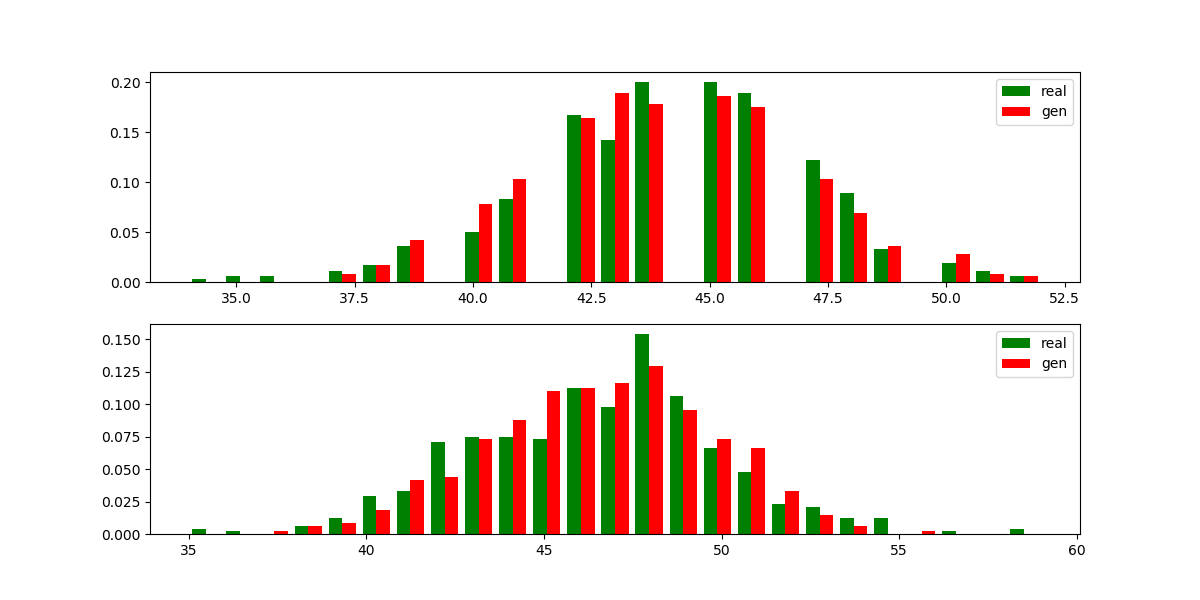
\includegraphics[scale = 0.18]{img/hist_comparison_[ 0.04 -0.08]_t_0.png}
        \includegraphics[scale=0.18]{img/hist_comparison_[  0.32 -0.52]_t_0.png}
    \end{center}
    \item $t = 3$:
        \begin{center}
        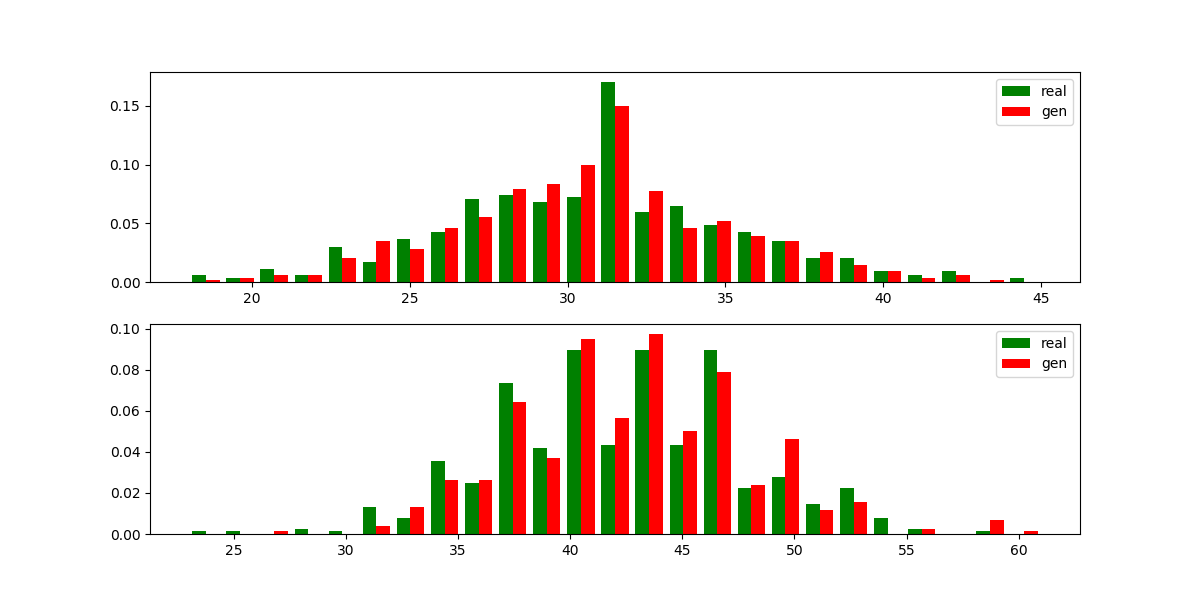
\includegraphics[scale = 0.18]{img/hist_comparison_[ 0.04 -0.08]_t_3.png}
        \includegraphics[scale=0.18]{img/hist_comparison_[  0.32 -0.52]_t_3.png}
    \end{center}
    \item $t = 15$:
        \begin{center}
        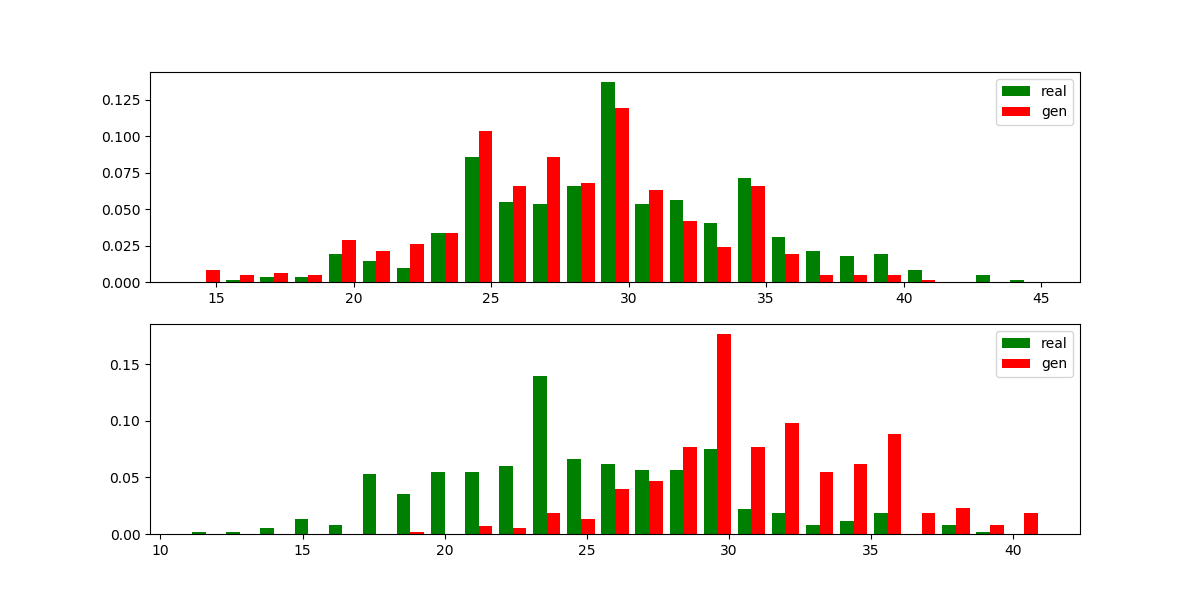
\includegraphics[scale = 0.18]{img/hist_comparison_[ 0.04 -0.08]_t_15.png}
        \includegraphics[scale=0.18]{img/hist_comparison_[  0.32 -0.52]_t_15.png}
    \end{center}
    \item $t = 31$:
        \begin{center}
        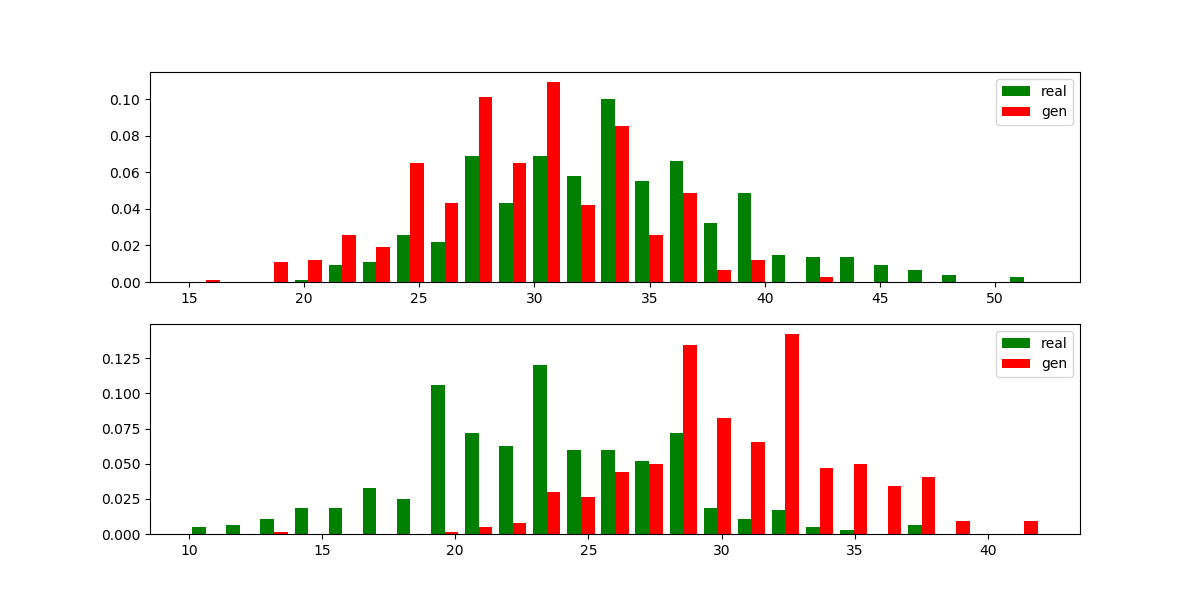
\includegraphics[scale = 0.18]{img/hist_comparison_[ 0.04 -0.08]_t_31.png}
        \includegraphics[scale=0.18]{img/hist_comparison_[  0.32 -0.52]_t_31.png}
    \end{center}
\end{itemize}

\begin{figure}[hb]
    \centering
    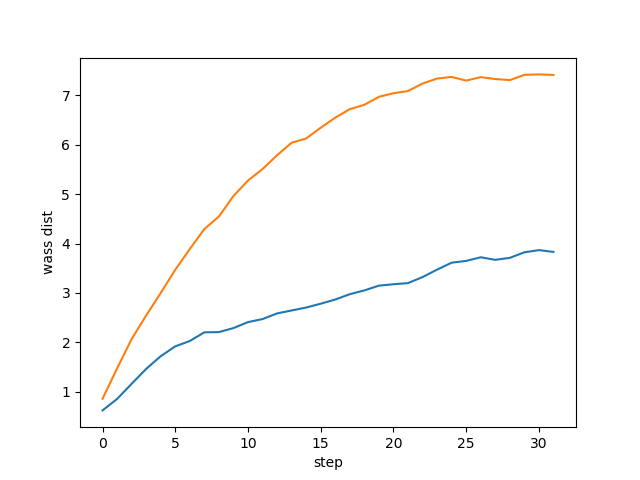
\includegraphics[scale = 0.4]{img/avg_wass_distance_32steps.png}
    \caption{Error propagation in using the approximated transition kernel to generate trajectories.}
    \label{fig:error_prop}
\end{figure}

We can observe a propagation of the error. In this regards we \textbf{propose} multiple \textbf{solutions}:
\begin{itemize}
    \item[(a)] try with WGAN rather then simple GAN;
    \item[(a)] enrich the dataset with all pairs $(s_t, s_{t+1})$ it will help in learning better the evolution towards the steady state;
    \item[(c)] learn the transition kernel for a single step but use a loss that measures the displacement in the generation of a trajectory of length $T$.
    
\end{itemize}

\textbf{Results} on the solutions proposed above:
\begin{itemize}
    \item[(a)] it is not straightforward to find the proper architecture for the WGAN;
    \item[(b)] as expected the propagation of the error is reduced as the training set contains more examples of the behaviour close to the steady-state scenario:
    \begin{center}
        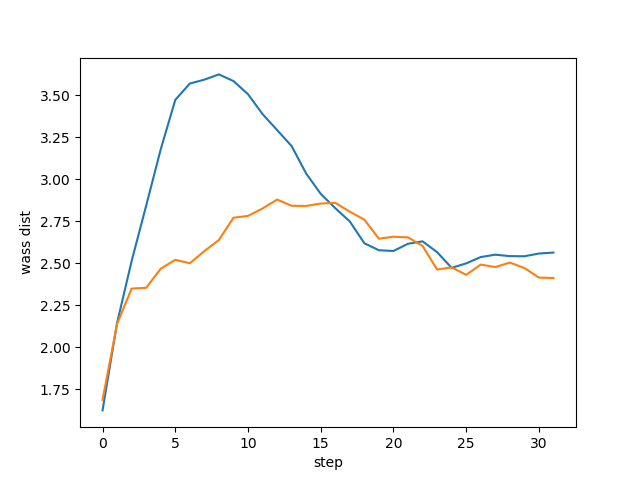
\includegraphics[scale = 0.4]{img/ENRICH_10ep_avg_wass_distance_32steps.png}
    \end{center}
    We observe a considerable reduction in the magnitude of the error (especially for species I (orange). The error, instead of constantly increasing, converges.
    
    \item[(c)] not that straightforward how to implement it in Tensorflow and not sure it would make a big difference compared to the trajectory approach.
\end{itemize}


TODO:

- what about other models? Show results.

- what about the scenario with varying parameters? Show results for eSIR with 1 parameter varying and with 3 parameters varying.


\section{Learn to generate a trajectory}

Given a state $s_0$, we can be represent the trajectory of length $T$ as a random variable over the state space $\mathcal{S}^T$. Dealing with inputs that are trajectories, i.e. sequences, requires the use of convolutive networks rather than feedforward. %We call this structure c-DCGAN (conditional-Deep Convolutional GAN).

In this regard, the Wasserstein GAN (WGAN) seems to work better than a normal GAN, especially regarding the mode collapse behaviour, i.e. when the GAN generates always the same trajectory, missing the stochastic behaviour of the system. 
In particular, the two networks are CNN and the WGAN is conditional. Therefore, we may call it a c-WCGAN (conditional-Wasserstein Convolutional GAN).

The GAN and the WGAN have some important differences that can be specified here (if needed). For example, the discriminator is a binary classifier in the GAN and a regressor, i.e. a critic, in the WGAN.

TODO: explain the main differences between GAN and WGAN.

\subsection{WGAN architecture}

The critic takes as input a trajectory of length $T+1$, as it contains the initial state as well, and it assign a critic value to it. 
\begin{lstlisting}
def define_critic():
	
	traj = Input(shape=(TRAJ_LEN+1, N_SPECIES)) 
		
	HC = [64, 64]
	KC = [4, 4]
	SC = [2,2]
	# weight constraint
	const = ClipConstraint(CLIP_CONST)
	# downsample 
	x = Conv1D(HC[0], KC[0], strides=SC[0], padding='same', kernel_constraint=const)(traj)
	x = BatchNormalization()(x)
	x = LeakyReLU(alpha=0.2)(x)
	# downsample 
	x = Conv1D(HC[1], KC[1], strides=SC[1], padding='same', kernel_constraint=const)(x)
	x = BatchNormalization()(x)
	x = LeakyReLU(alpha=0.2)(x)

	# scoring, linear activation
	x = Flatten()(x)
	outputs = Dense(1)(x)
	x = Dropout(0.4)(x)

	model = Model(inputs=traj, outputs=outputs)

	# compile model
	opt = RMSprop(lr=C_LR)
	model.compile(loss=wasserstein_loss, optimizer=opt)

	return model
\end{lstlisting}
The generator takes as input the initial state and a noise value and generates as output a trajectory of length $T$, which can be passed as input to the critic.

Two alternative approaches to reshape the inputs. The noise, that initially has shape $(latent\_dim)$, is mapped into an array of shape $(Q,N\_CH)$, where $Q$ is related to the number of upsampling layers present in the generator CNN, $n\_hidden\_gen$. In particular, $Q = TRAJ\_LEN/n\_hidden\_gen$.
\begin{lstlisting}
def define_generator(latent_dim):
	
	noise = Input(shape=(latent_dim)) 
	n_nodes_n = N_CH * Q
	nv = Dense(n_nodes_n)(noise)
	nv = Reshape((Q, N_CH))(nv)

	init_states = Input(shape=(N_SPECIES))
	
	if embedding== "DENSE":
		n_nodes_i = Q * 1
		iv = Dense(n_nodes_i)(init_states)
		iv = Reshape((Q, 1))(iv)
	else:
		iv = RepeatVector(Q)(init_states)

	merge = Concatenate(axis=2)([iv,nv])

	HG = [128, 256, 128]
	KG = [4, 4, 4, 4]
	SG = [2, 2, 2]
	# upsample to 2*Q = 8
	x = Conv1DTranspose(HG[0], KG[0], padding = "same", strides = SG[0])(merge)
	x = BatchNormalization()(x)
	x = LeakyReLU(alpha=0.2)(x)
	
	# upsample to 4*Q = 16
	x = Conv1DTranspose(HG[1], KG[1], padding = "same", strides = SG[1])(x)
	x = BatchNormalization()(x)
	x = LeakyReLU(alpha=0.2)(x)
	
	# upsample to 8*Q = 32
	x = Conv1DTranspose(HG[2], KG[2], padding = "same", strides = 2)(x)
	x = BatchNormalization()(x)
	x = LeakyReLU(alpha=0.2)(x)
	
	# output
	outputs = Conv1D(N_SPECIES, KG[-1], activation='tanh', padding='same')(x)
	print("GEN OUTPUT: ", outputs)

	model = Model(inputs=[noise,init_states], outputs=outputs)
	return model

def define_gan(generator, critic):
	# make weights in the critic not trainable
	critic.trainable = False
	noise, init_states = generator.input
	gen_traj = generator.output

	in_st = Reshape((1,N_SPECIES))(init_states)
	merged_traj = Concatenate(axis=1)([in_st, gen_traj])

	gan_output = critic(merged_traj)

	model = Model(inputs=[noise, init_states], outputs=gan_output)

	# compile model
	opt = RMSprop(lr=G_LR)
	model.compile(loss=wasserstein_loss, optimizer=opt)
	return model
\end{lstlisting}

\subsection{Results}

\subsubsection{Ergodic SIR model}
The results for the eSIR model are promising and shown in Figure~\ref{fig:esir_trajectories}. Six validation points, i.e., initial states, are chosen. Each point is represented by a pair of trajectories, the top one is for species S and the bottom one is for species I.
\begin{figure}[hb]
    \centering
    \subfigure[]{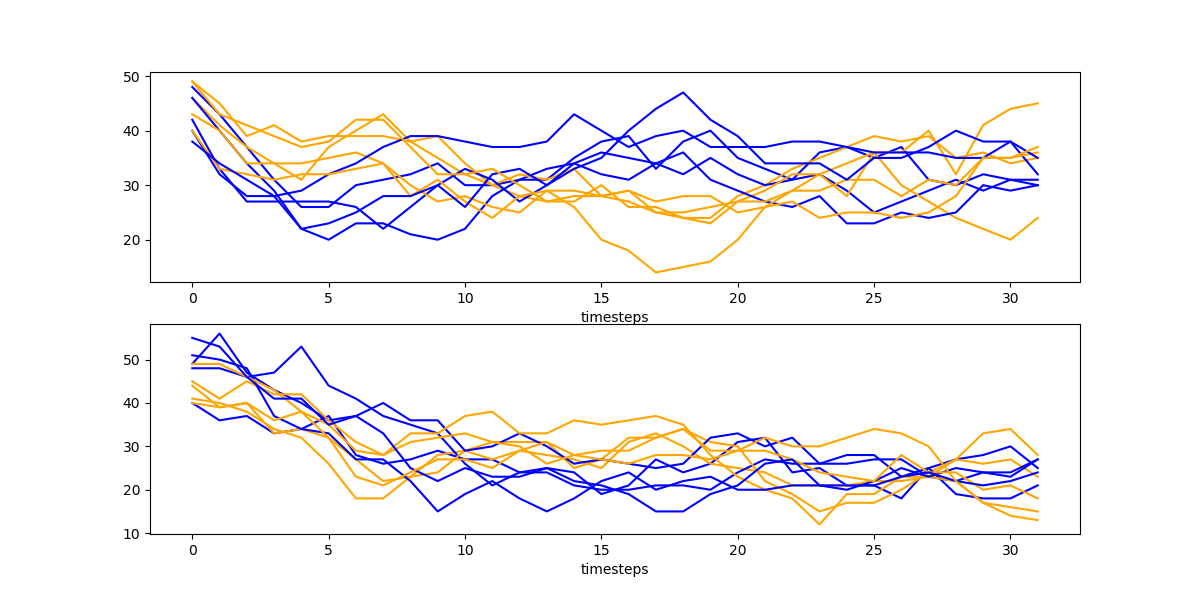
\includegraphics[scale = 0.19]{img/eSIR_Trajectories0.png}}
    \subfigure[]{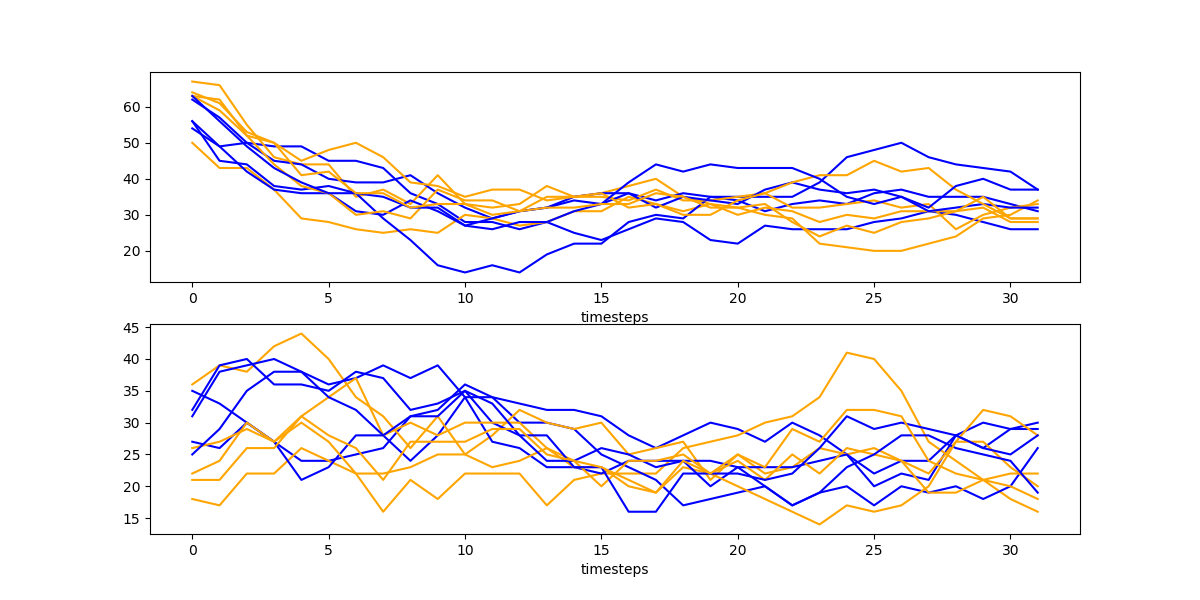
\includegraphics[scale = 0.19]{img/eSIR_Trajectories1.png}}
    \subfigure[]{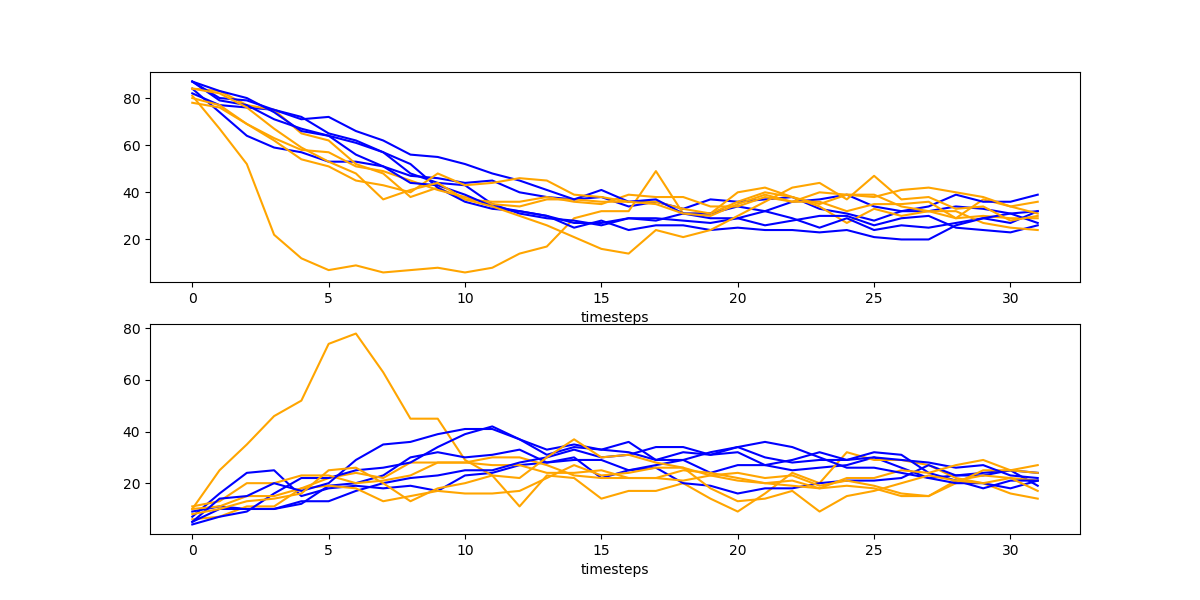
\includegraphics[scale = 0.19]{img/eSIR_Trajectories4.png}}
    \subfigure[]{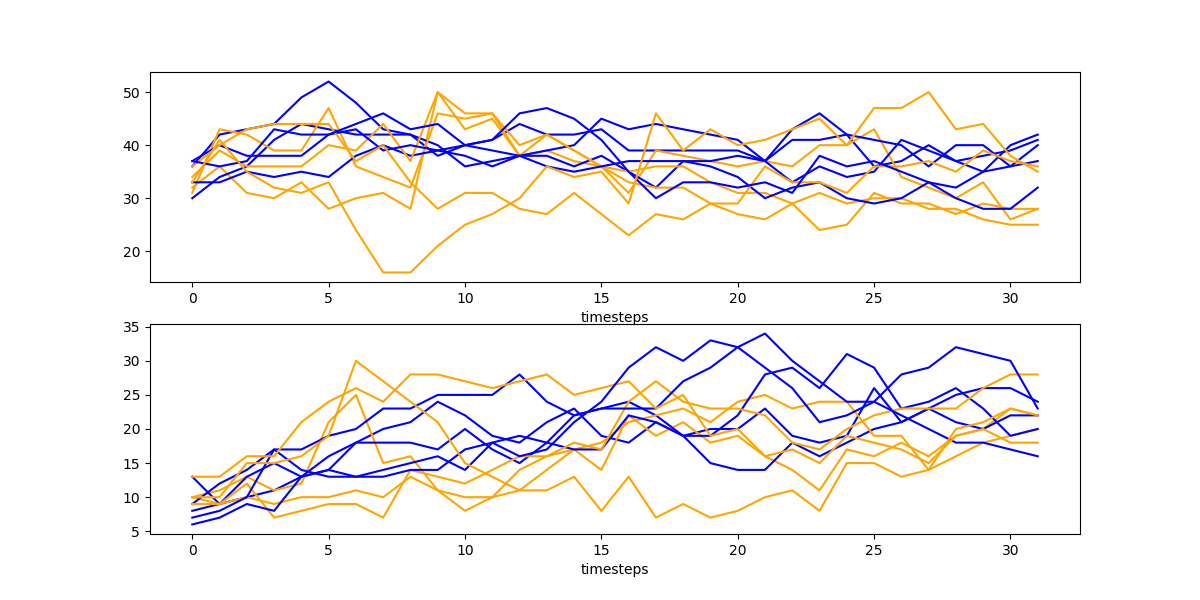
\includegraphics[scale = 0.19]{img/eSIR_Trajectories5.png}}
    \subfigure[]{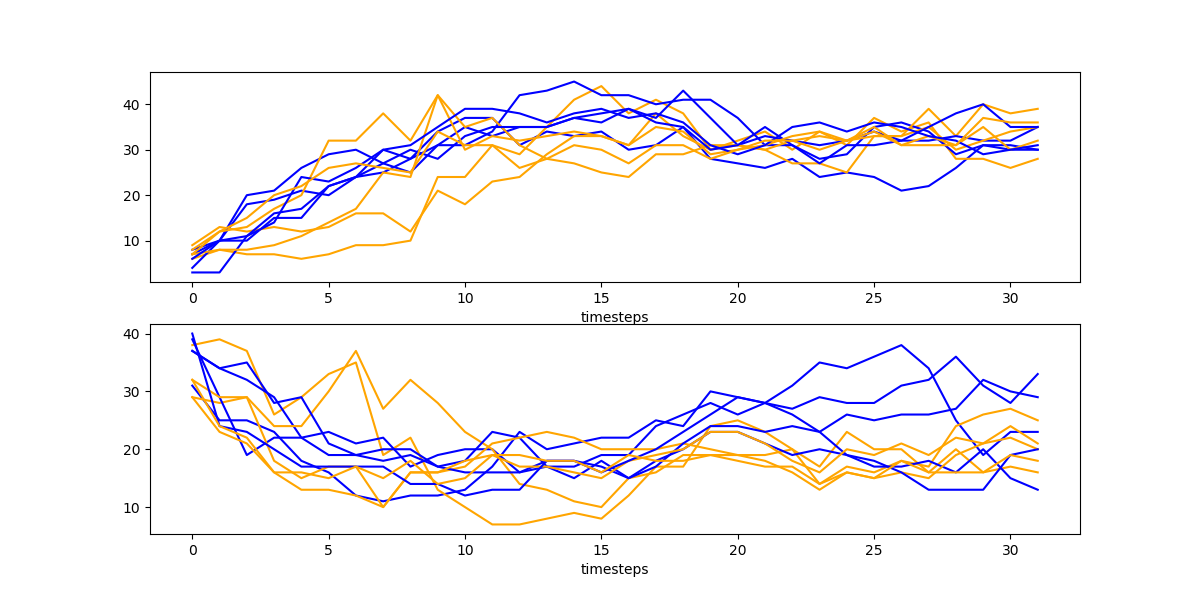
\includegraphics[scale = 0.19]{img/eSIR_Trajectories8.png}}
    \subfigure[]{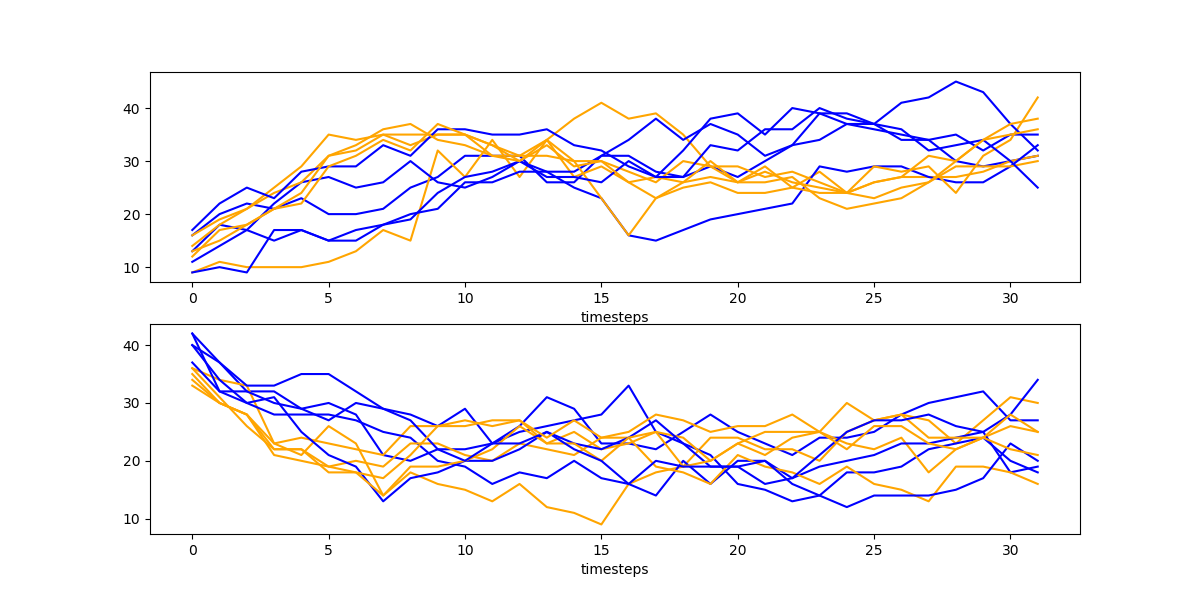
\includegraphics[scale = 0.19]{img/eSIR_Trajectories9.png}}
    \subfigure[Average Wasserstein distance.]{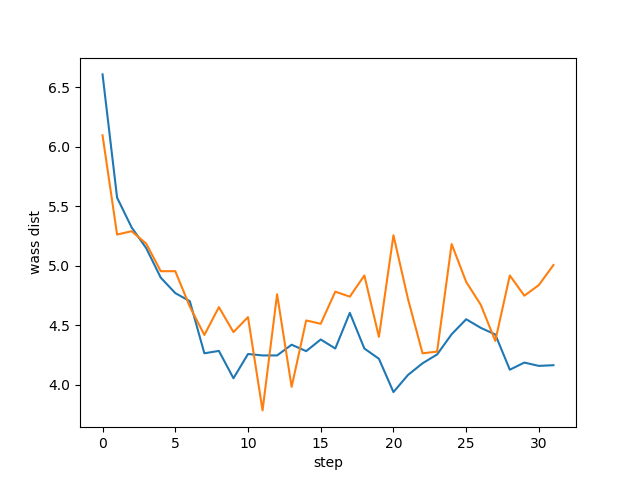
\includegraphics[scale = 0.4]{img/eSIR_traj_avg_wass_distance.png}}
    \caption{eSIR model: comparison of trajectories generated with a WGAN (orange) and the trajectories generated with the SSA algorithm (blue).}
    \label{fig:esir_trajectories}
    
    
\end{figure} 

\subsubsection{Toggle Switch model: bistability}
The results for the TS model are shown in Figure~\ref{fig:ts_trajectories}. The GAN works well on the trajectories of the proteins, i.e., it is able to capture the bistale beahaviour. This means that we are ignoring the state of the genes. If we take them into account the method does not work. Probably harder to learn the binary trajectories.

\begin{figure}[hb]
    \centering
    \subfigure[]{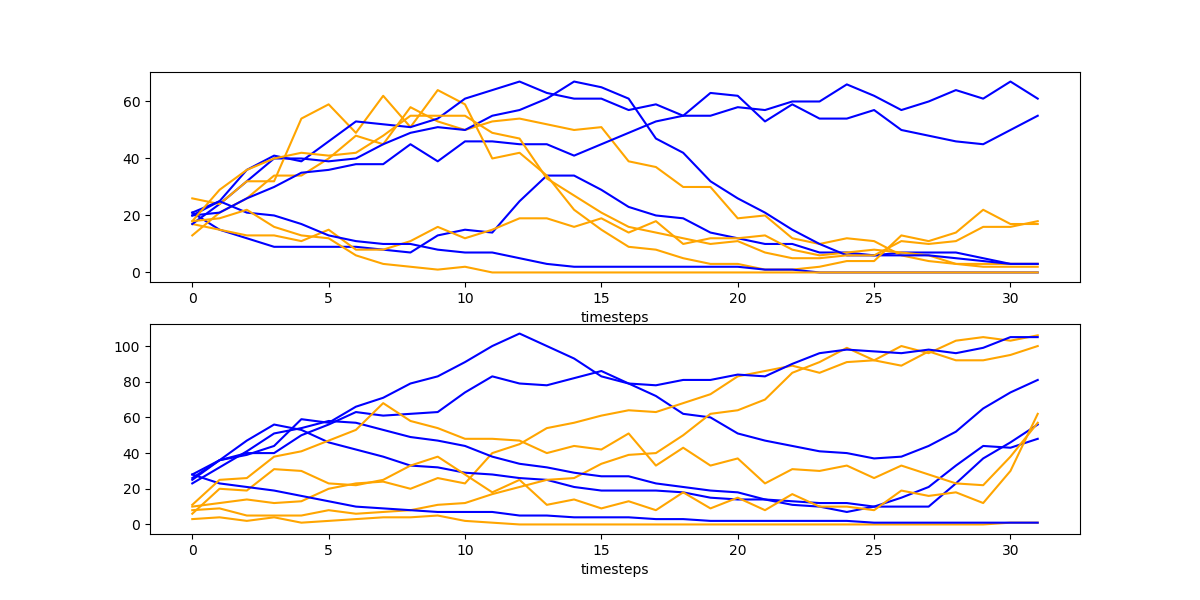
\includegraphics[scale = 0.19]{img/Trajectories0.png}}
    \subfigure[]{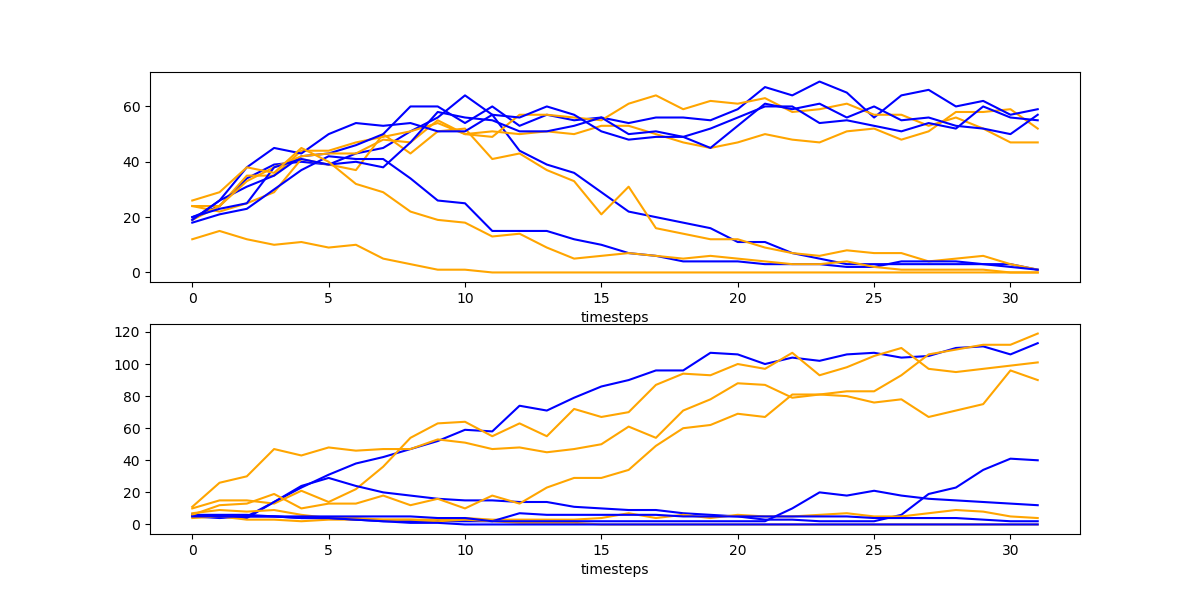
\includegraphics[scale = 0.19]{img/Trajectories1.png}}
    \subfigure[]{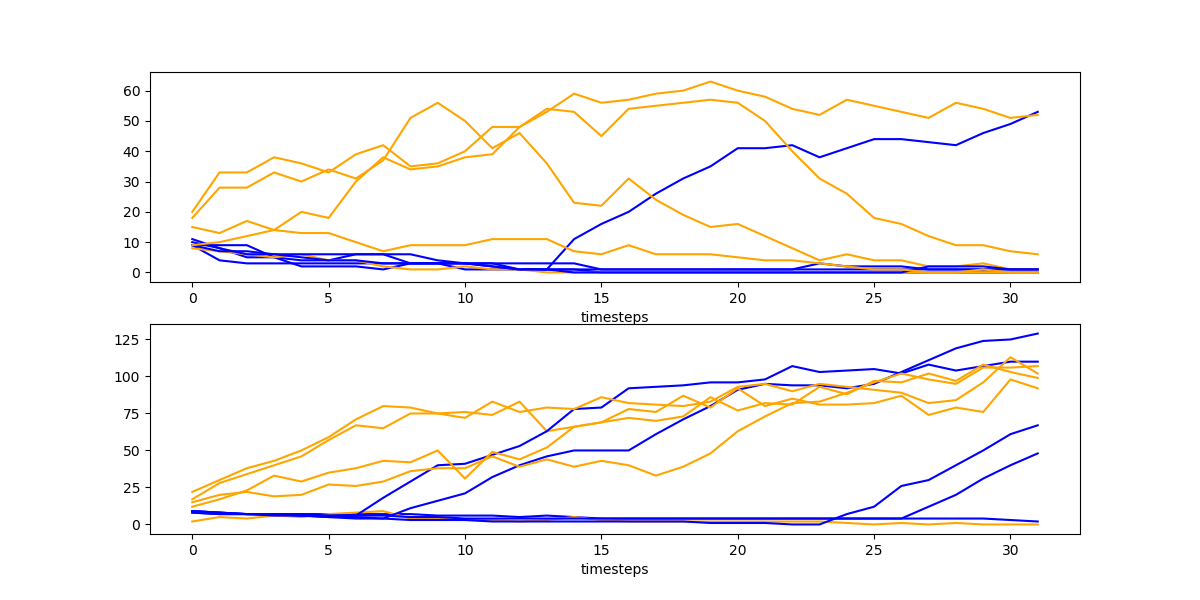
\includegraphics[scale = 0.19]{img/Trajectories4.png}}
    \subfigure[]{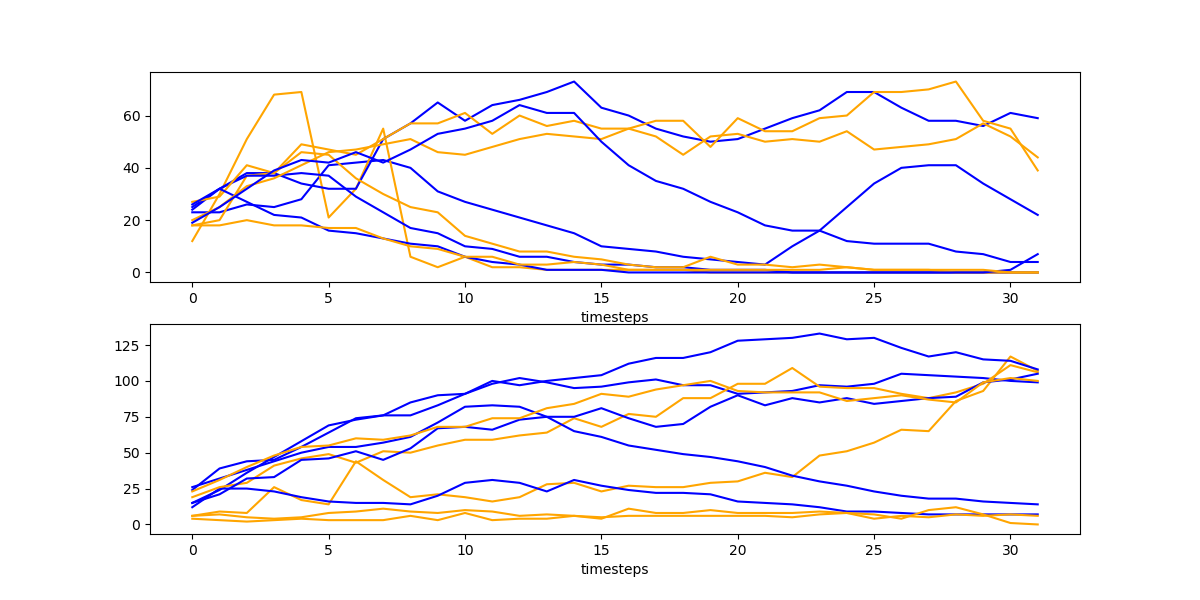
\includegraphics[scale = 0.19]{img/Trajectories5.png}}
    \subfigure[]{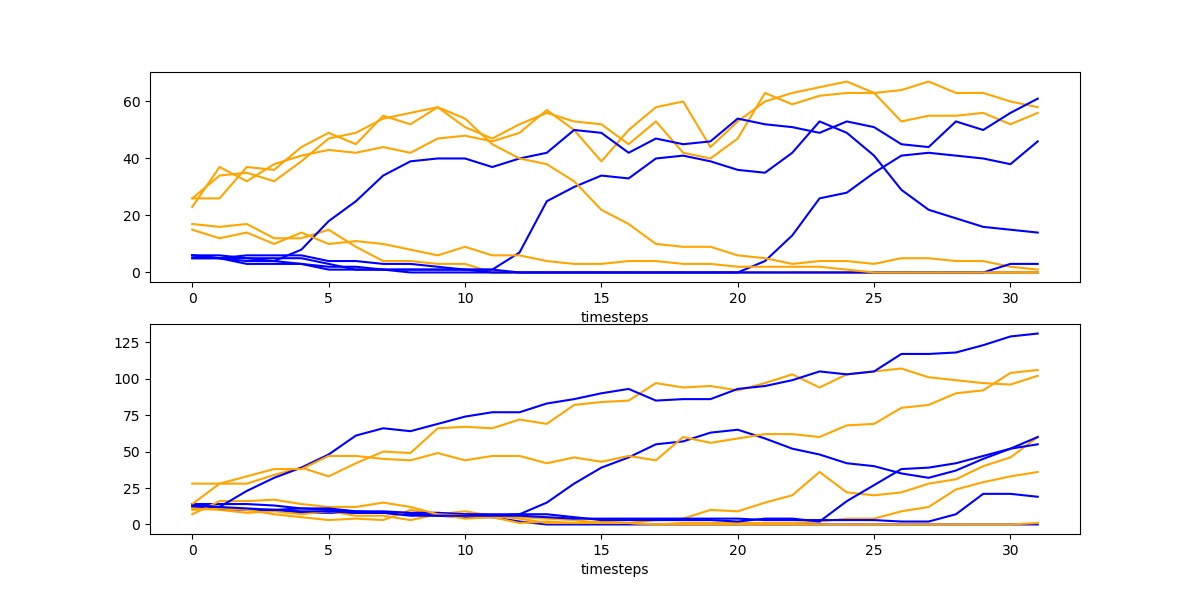
\includegraphics[scale = 0.19]{img/Trajectories8.png}}
    \subfigure[]{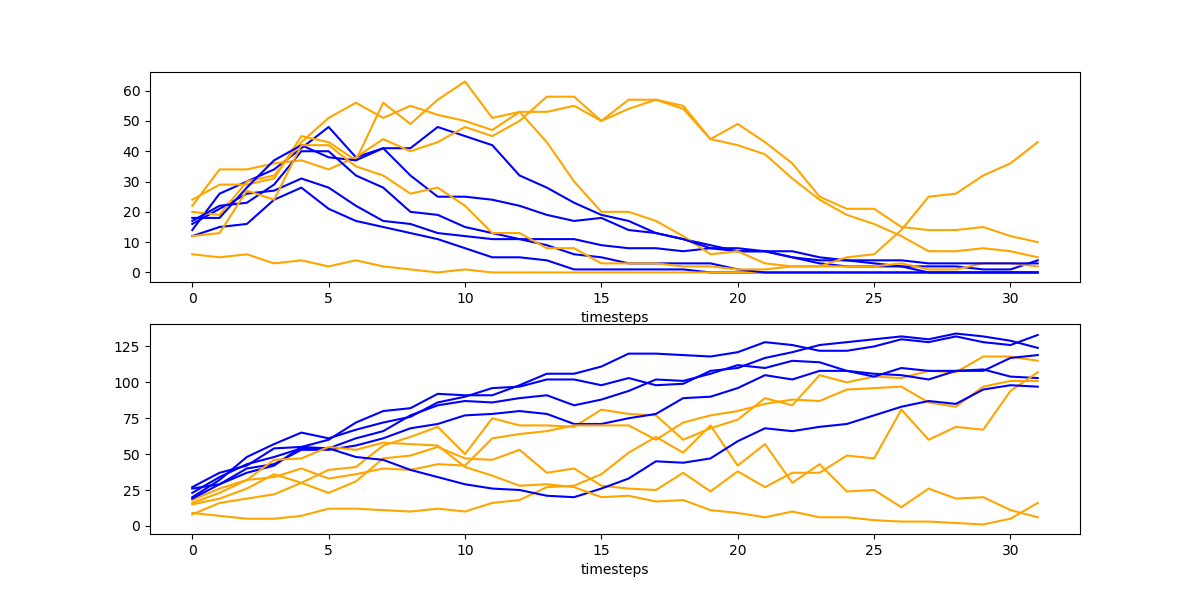
\includegraphics[scale = 0.19]{img/Trajectories9.png}}
    \caption{eSIR model: comparison of trajectories generated with a WGAN (orange) and the trajectories generated with the SSA algorithm (blue).}
    \label{fig:ts_trajectories}
\end{figure} 

   
    
\section{Learning the steady state distribution with unconditional GAN}

Simpler scenarios in which the time interval is large enough to reach the steady state. Therefore, the distribution is independent on the initial state, and so a simple unconditioned GAN (or WGAN) is sufficient to approximate it.

In the steady state the behaviour may look extremely multi-modal, as for example in the GRN model.

\begin{figure}
    \centering
    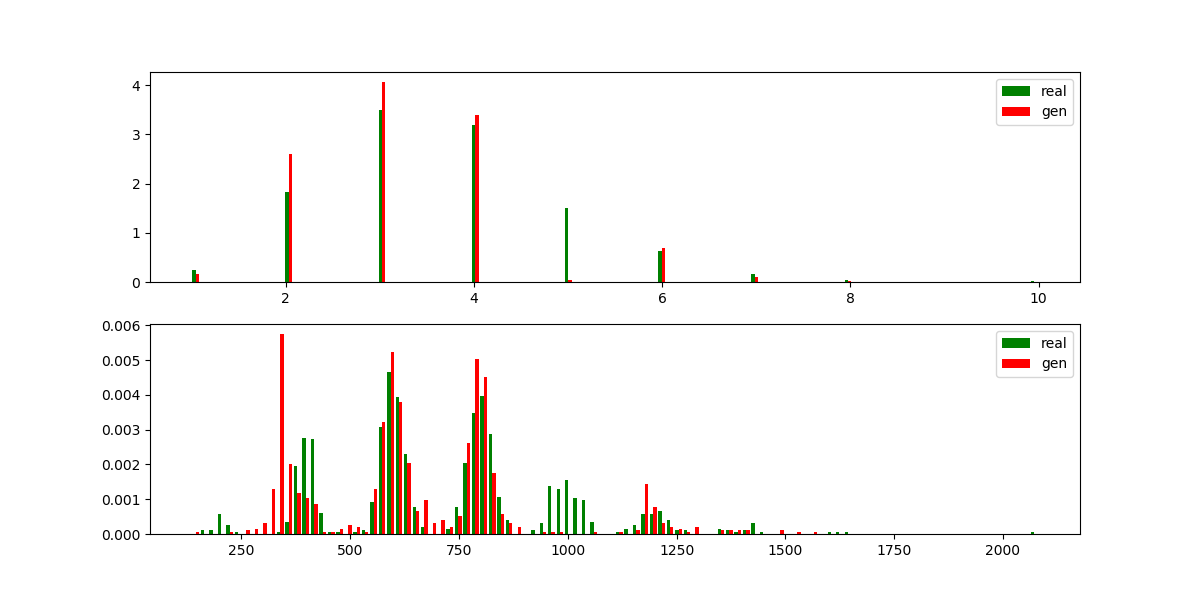
\includegraphics[scale = 0.4]{img/GRN_steady_state.png}
    \caption{Approximation of the steady state distribution of the GRN model with a GAN.}
    \label{fig:GRN_ss}
\end{figure}

Details of the actual architecture: 
\begin{itemize}
    \item Leaky ReLU activation with 0.2 slope, no batch normalization;
    \item learning only the distribution of mRNA and proteins;
    \item 5 hidden layers with 10 neurons each fort both the disctiminator and the generator;
    \item 300 epochs; iteration ratio 1 disriminator for 30 generator updates; noise dimension 200; learning rates $10^{-4}$ for the discriminator and $10^{-6}$ for the generator.
\end{itemize}

%\bibliographystyle{plain}
%\bibliography{references}
\end{document}
